\documentclass{beamer}
\usepackage{xcolor}
\usepackage{fontspec}


% Standard colors
\definecolor{Red}{rgb}{1,0,0}
\definecolor{Blue}{rgb}{0,0,1}
\definecolor{Green}{rgb}{0,1,0}
\definecolor{Orange}{rgb}{1,0.65,0}
\definecolor{Black}{rgb}{0,0,0}

% Custom hex-based colors
\definecolor{DeepAquamarine}{HTML}{78DBE2}
\definecolor{DeepBlush}{HTML}{E36F8A}
\definecolor{DeepSaffron}{HTML}{FF9932}

% Set theme and colors
\setbeamercolor{background canvas}{bg=white}
\setbeamercolor{title}{fg=Blue}
\setbeamercolor{frametitle}{fg=Orange}
\setbeamercolor{normal text}{fg=Black}

% Fonts
\setmainfont{Times New Roman} % Default font for English
\newfontfamily\oriyafont{Odia Archana} % Font for Odia text

\begin{document}

% Slide 1: Title Slide
\begin{frame}
    \begin{center}
        \color{Orange}\Huge The Scientific Method\\
        \vspace{0.5cm}
        \color{Blue}\large \oriyafont ବୈଜ୍ଞାନିକ ପଦ୍ଧତି
    \end{center}
\end{frame}

% Slide 2: Lack of Basic Infrastructure
\begin{frame}
    \frametitle{\color{Orange}\oriyafont ପ୍ରଶ୍ନ ଉଠାଇବା  ଏବଂ ବିଜ୍ଞାନ-ଭିତ୍ତିକ ଉତ୍ତର ଖୋଜିବା }

 
- \color{Black} \oriyafont ଜୀବବିଜ୍ଞାନୀମାନେ ଜୀବ ଜଗତ ବିଷୟରେ ପ୍ରଶ୍ନ ଉଠାଇ ଏବଂ ବିଜ୍ଞାନ-ଭିତ୍ତିକ ଉତ୍ତର ଖୋଜି ଅଧ୍ୟୟନ କରନ୍ତି। ଏହି ପଦ୍ଧତି ଅନ୍ୟାନ୍ୟ ବିଜ୍ଞାନ ପାଇଁ ମଧ୍ୟ ସାଧାରଣ ଏବଂ ଏହାକୁ ପ୍ରାୟତଃ ବୈଜ୍ଞାନିକ ପଦ୍ଧତି ଭାବରେ କୁହାଯାଏ। ବୈଜ୍ଞାନିକ ପଦ୍ଧତି ପ୍ରାଚୀନ କାଳରେ ମଧ୍ୟ ବ୍ୟବହୃତ ହେଉଥିଲା, କିନ୍ତୁ ଏହାକୁ ପ୍ରଥମେ ଇଂଲଣ୍ଡର ସାର୍ ଫ୍ରାନ୍ସିସ୍ ବେକନ୍ (1561-1626) (ଚିତ୍ର 1.5) ଦ୍ୱାରା ଦଲିଲ କରାଯାଇଥିଲା, ଯିଏ ବୈଜ୍ଞାନିକ ଅନୁସନ୍ଧାନ ପାଇଁ ଆଗମନାତ୍ମକ ପଦ୍ଧତି ସ୍ଥାପନ କରିଥିଲେ।


\end{frame}

% \begin{figure}[h!]
%     \centering
%     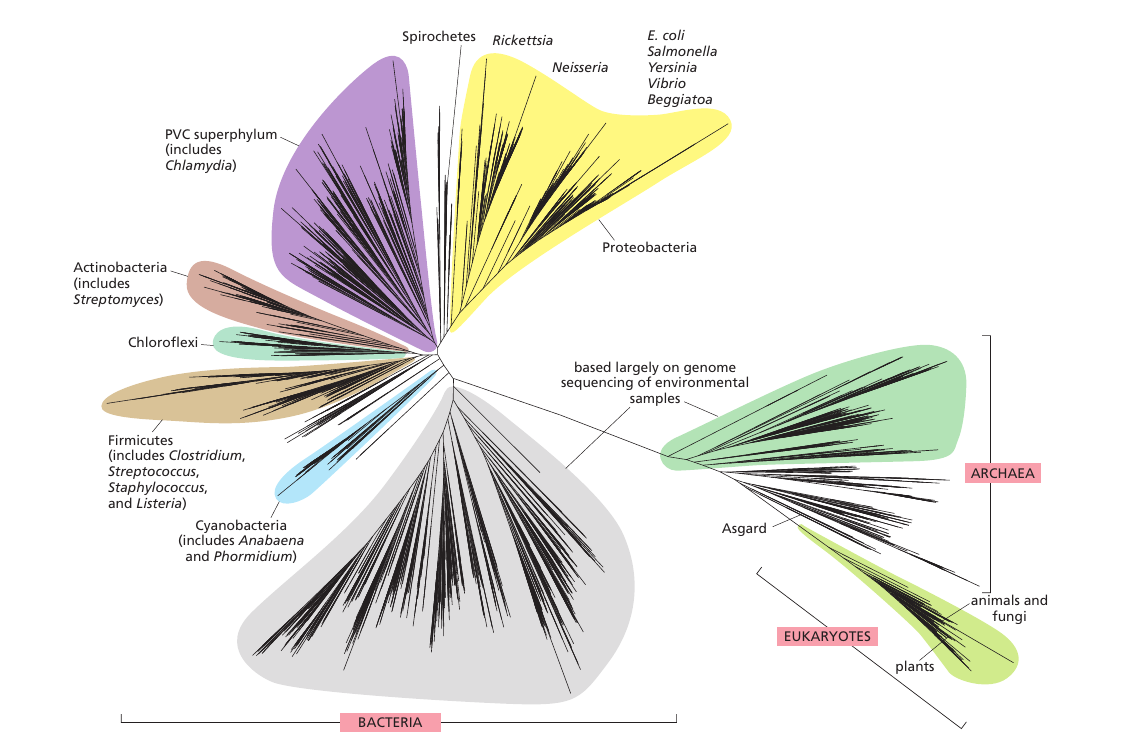
\includegraphics[width=0.9\textwidth]{domains.png} % Replace with your image file name
%     \caption{\oriyafont ଜୀବ ଜଗତର ତିନୋଟି ପ୍ରମୁଖ ବିଭାଗ (ଡୋମେନ୍, domain)}
%     \label{fig:sample-image}
% \end{figure}

\end{document}
